\section{Data}

In this thesis two different data sets will be used; the well-studied MNIST data set \cite{MNIST} of handwritten digits, and the relatively new THETIS data set \cite{Gourgari2013} of videos of tennis shots. The idea is to first apply the methods discussed later to the simpler MNIST data set, to make sure that it is working properly, followed by an application to the more complicated THETIS data set. Each of the data set will be described in the following. 

\subsection{MNIST - Handwritten digits}
The MNIST (Modified National Institute of Standards and Technology) data set \cite{MNIST} consists of 70,000 pictures\footnote{The 70,000 is split into 60,000 training pictures and 10,000 testing pictures} of handwritten digits from 0 through 9. Each picture is $28\times 28$ pixels and black/white which means that there is only one input channel. Each of the $28\cdot 28 = 784$ pixel values are intensities ranging from 0 (black) to 255 (white). The data set is formed by remixing samples from the earlier NIST data set, which consisted of both digits and characters. The MNIST samples would be picked out, standardized and normalized so they would all be the same size and have the same gray-values \cite{mnistdatabase}. The first 200 samples from the traning set of the MNIST database is shown in \autoref{fig:MNISTdata200}. 

\begin{figure}[ht]
    \centering
    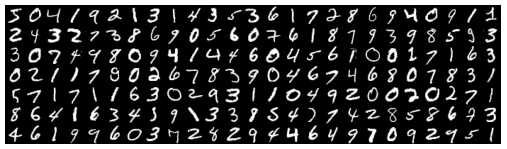
\includegraphics[width=\linewidth]{Pics/04_Data/MNIST.png}
    \caption{The first 200 samples of the MNIST data set of handwritten digits}
    \label{fig:MNISTdata200}
\end{figure}

\subsection{THETIS - Tennis shot videos}
